\documentclass{article}

\usepackage{amsmath} % For gather and other math environments
\usepackage{setspace} % For double spacing
\usepackage{mathtools} % amsmath extensions
\usepackage{amsfonts} % math fonts
\usepackage{graphicx} % for images
\usepackage{listings} % for code blocks
\usepackage{color}    % for colored code
\usepackage{pgfplots} % for plotting function
\usepackage{booktabs} % for tables
\usepackage{float}
\usepackage{algorithm} % for algorithm notation
\usepackage{algpseudocode}

\usepackage[a4paper, margin=3.17cm]{geometry}

\graphicspath{{ ./images/ }}

\begin{document}

\begin{titlepage}
    \vspace*{\fill}
    \vspace*{-4cm}
    \begin{center}
        \huge \textbf { Deep Reinforcement Learning: An Application to Single-machine Batch Job Scheduling } \\
        \vspace{0.5cm}
        \Large \textit { by Filip Toth }
    \end{center}
    \vspace*{\fill}
    \begin{center}
        \large \textit {An IB Extended Essay in the subject of Computer Science}
    \end{center}
\end{titlepage}

\tableofcontents
\newpage

\begin{spacing}{2.0}

\section{Introduction}

High Performance Computing (HPC) is almost everywhere in modern the software development life-cycle and consumption. We use it to train neural networks, efficiently price
financial assets, perform large-scale data mining and user data harvesting operations, run modern DevOps workflows, predict weather patterns, validate semiconductor designs
for flaws, optimize just-in-time manufacturing processes, and so much more. The global HPC market is valued at $52.56$ billion and is poised to grow to $87.31$ billion by 2030
at a CAGR of 7.5[source - will be converted to proper citing later](https://www.grandviewresearch.com/industry-analysis/high-performance-computing-market). This presents an
enormous opportunity to rethink and optimize the world's computing infrastructure. The backbone of these HPC systems are non-AI enabled workload managers such as SLURM or PBS.
In this extended essay we inquire whether reinforcement learning-based machine learning models can be used to create a more optimized batch job scheduler. Our system will also
be more flexible, the ML model can be trained to put more emphasis on a specific scheduling metrics, which with current systems requires a large amount of configuration and is
still limited by internal heuristics. Although we currently only work in the context of a single node cluster, this can easily be extended to multiple nodes and might also
provide for more synergies especially alleviating single-node resource fragmentation, since the allocation of which nodes handle which process groups can also be optimized by
the ML model, it's all a variation of the basic knapsack problem, just applied at different scales. It's also worthwhile to mention that this is an active area of research,
and such systems have already been created and partially deployed. Hongzi Mao et al. at the Massachusetts Institute of Technology along with Microsoft Research were among
the earliest pioneers of this technology and have successfully devised a reinforcement learning-based system that outperforms current heuristics on batch job scheduling.
Their paper has definitely played a key role in influencing our research especially with some of the clever tricks used to model the job basket as an input to the neural network.

\newpage
\section{An Overview of the Problem of Single-Machine Process Scheduling}

Considering a set of jobs $J_{1}, J_{2}, \cdots J_{n}$ that need to be run on a system sequentially, what is the most efficient way to run these processes such that the can experience the lowest amount of resource-space downtime due to the unused resources and utilize the system's parallelization capabilities to the fullest extent. In a simplified, yet very useful overview, processes have two discrete parameters: CPU-time requirements and memory requirements. We generally evaluate scheduling algorithms based on the following criteria:

\begin{itemize}
    \item Job Throughput - execute the highest number of processes per unit time.
    \item Turnaround Time - minimize the duration from when the job is submitted to its completion.
    \item Maximize Resource Utilization
\end{itemize}

Note that in this micro-view of scheduling on a single node rather than a large cluster, the execution plane becomes $2$ dimensional and multiple jobs
can be executed in the same time-frame, leaving short-term scheduling up to the CPU, this also works to increase resource utilization. We would consider
resources to have a dimension in our resource use matrix, and time, is the other dimension of course, since we know the allotted running time of each batch
job and need to represent compute time in some way. E.g. we consider a compute node with $m$ memory and $c$ CPU cores, the resource use matrix for this
matrix would be in the following vector space: $\mathcal{R} \in \mathbb{R}^{(m + c) \times t}$, where $t$ is the time dimension.

\newpage
\section{An Overview of Current Heuristics}

So how do modern batch schedulers and workload managers like SLURM or OpenPBS solve this problem?

\begin{itemize}
    \item \textbf{First Come, First Serve} - the simplest algorithm implementation-wise, it's implemented through a basic queue, nothing else is taken into consideration.
    Its performance is quite poor.

    \item \textbf{Shortest Job First (SJF)} - This algorithm executes the shortest jobs first from the set of available jobs. This works to reduces average waiting
    times and maximizes job throughput, but also causes the problem of starvation where longer jobs may never be executed even if they've been submitted to the
    waiting queue. Historically, SJF has been implemented using multiple different queues based on job length and SJF would run on each of these queues separately,
    for example having a separate queue for short jobs, medium jobs and long jobs. This partially solves the problem of starvation, while still improving performance.

    \item \textbf{Bin Packing Scheduler} - Also sometimes referred to as a Tetris scheduler. This algorithm utilizes the bin packing problem (although since we
    only have "one bin", it more closely relates to the knapsack problem) to run more jobs at the same time without causing resource conflicts. This works to
    maximize resource utilization.
\end{itemize}

Modern schedulers utilize a combination of these algorithms to achieve a balance between all criteria and metrics. Schedulers are also often times tweaked for
the client's specific project needs. This can also be done in our ML model through the introduction of a coefficient to each of the reward signals.

\newpage
\section{A Deeper Look into Scheduling Optimization Metrics}

\textbf{Mean Slowdown:} this is one of the most important metrics in job scheduling optimization. It measures the time that a job has been waiting plus the execution time over its real execution time. It's defined as:

\begin{gather*}
    \overline{S} = \frac{1}{n} \sum_{i = 1}^{n} \frac{t^{real}_{i} + t^{wait}_{i}}{t^{real}}
\end{gather*}

where $t^{real}_{i}$ is the execution time of the job, and $t^{wait}_{i}$ is the waiting time for the job to begin execution. A problem arises in practice when we consider very short-running jobs, their waiting time has a much higher impact on the overall metric. Factoring this in, we get the bounded mean slowdown, defined as:

\begin{gather*}
    \overline S_{b} = \frac{1}{n} \sum_{i = 1}^{n} max \left (\frac{t_{i}^{real} + t_{i}^{wait}}{max(t_{i}^{real}, \tau)}, 1 \right )
\end{gather*}

where $\tau$ is an arbitrary constant that ensures that creates an upper bound for the maximum real time that gets considered.

\textbf{Response Time:} this is a very basic metric solely focusing on the time the job has been in the system, although it can become very useful as a minimization reward proxy when training the model. It's defined as:

\begin{gather*}
    \mathcal{RT} = \frac{1}{n} \sum_{i = 1}^{n} t^{real}_{i} + t^{wait}_{i}
\end{gather*}

\textbf{Utilization:} this metric measures the work that has been performed by job processes on the system v.s. the number of total possible work that can theoretically be done on the system between a specified time interval. It can be thought of as the packedness of system resources. It's defined as:

\begin{gather*}
    U(t_{1}, t_{2}) = \frac{W(t_{1}, t_{2})}{N \cdot (t_{2} - t_{1})}
\end{gather*}

where $t_{1}$ is the starting time of the measurement and $t_{2}$ is the ending timestamp of the measurement, $W(t_{1}, t_{2})$ is the total amount of work done between $t_{1}$ and $t_{2}$, and $N$ is the number of utilizable resources in the system. Note that in our case where this metric will be converted to a reward for the reinforcement learning algorithm, $t_{1}$ will always be zero.

\newpage
\section{A Rundown of Deep Reinforcement Learning (Deep RL)}

In RL (reinforcement learning), we use iterative interaction with the environment model to optimize a policy $\pi$ such that the maximizes reward and the expected value
of the policy $\mathbb{E}_{\pi}$, a policy that maximizes this value and converges is called the optimal policy $\pi_{*}$. Supervised learning models work as maps
$f: \mathbb{R}^{n} \rightarrow \mathbb{R}^{m}$ between features and labels. RL, on the contrary, learns a policy that then scholastically chooses an action
from a probability distribution, they can also take a series of actions. Most RL models essentially run through a time-series where $t$ is the time step of
the current state. The agent (the model we're training) makes takes an action based on the accumulated discounted return $R_{t} = \sum\limits_{k = 0}^{\infty} \gamma^{k} r_{t + k}$,
where the discount factor $\gamma \in [0, 1)$ controls how important is future vs immediate reward. This is defined by the model's policy (it's behavior function)
$\pi \left ( a | s \right )$ which maps a state to an action that the agent undertakes. In our case, this function is partly stochastic (non-deterministic).
After the agent takes an action, we proceed to the next time-step and next state $s_{t + 1}$ determined stochastically by the state transition probability
$\mathbb{P}(s_{t + 1} | s_{t}, a_{t})$. Training an RL model can be generalized into:

\begin{gather*}
    \underset{\pi}{argmax} \hspace{0.5cm} \underset{a_{t} \sim \pi(\cdot |s_{t}), s_{t + 1} \sim \mathbb{P} (\cdot | s_{t}, a_{t})  }{\mathbb{E}} \left [ \sum\limits_{t = 0}^{\infty} \gamma^{t} r(s_{t}, a_{t}) \right ]
\end{gather*}

In this specific application of RL, we'll use deep Q-learning and deep Q-networks (DQNs). In traditional Q-learning, a map would be constructed from each state-action
pair to a Q-value following a policy, where this Q-function maps to the expected returns following the supplied action under a specific state,
$Q^{\pi}(s, a) = \mathbb{E}_{\pi} \{ G_{t} | s_{t} = s, a_{t} = t \}$. In deep Q-learning, we use two DQNs to approximate this Q-function and converge on a
locally optimal policy. We use a policy DQN and a target DQN, each with the same model architecture. The policy network serves to make approximate the Q-function and
pick state-action pairs for the actor to perform, while the target network learns from the experience replay buffer to compute the loss for the policy network.
A smooth L1 Hubert loss is computed at the end of each training pass and back-propagated through the network. At the end of each training epoch, random state-action pairs
are selected and propagated through the policy network and stored in the experience replay buffer, and are then used as training data for the target network.

\begin{center}
    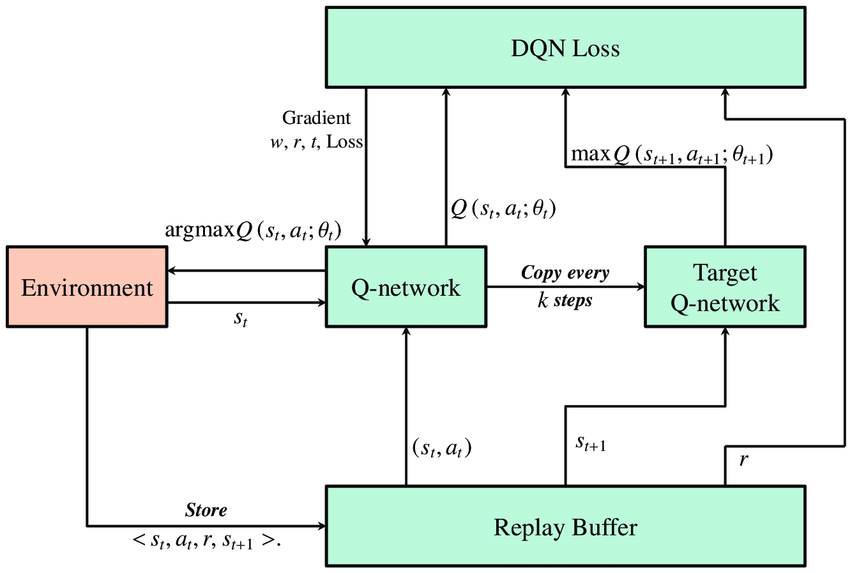
\includegraphics[scale=0.35]{./images/A-Concept-of-DQN-Algorithm7.png}
\end{center}

\newpage
\section{Modelling the Environment}

A basic structure of our environment model is the Job. The job can be represented as a struct describing the properties of the job - mainly the start time-step, the
length of the job, and allocated resources. All of these are then passed on as inputs to both the policy and target DQNs. For each action the actor can assume in
every state, our environment has to return an observation (next state that the actor then assumes in the next time step), a reward after taking the action, and a
boolean value indicating whether the action taken has "ended the game" (terminated), i.e. whether the next state the model can assume is null.

Our specific environment will model the inner workings of a batch-job worker. The worker (assuming a singular machine system) has a matrix to store resource use for
each of the future time steps. When a time step passes, the resource use matrix truncates its zero-th element and the jobs that have finished running. Note that resources
need to be finite for the actor to be able to correctly process the reward value functions for state-action pairs.

As the actor (training policy network) interacts with the environment, the actor is tasked with selecting an action from a discrete (i.e. non-continuous)
action space $\mathcal{A} = \{ 0, 1, \cdots n + 1 \}$ where $n$ is the size of the job queue exposed in the observation tensor. Each member of the action
represents the index of a job slot to be scheduled. The environment then loads the job from the job slot and performs a check whether the job can be scheduled
within our machine resource matrix. If the job cannot be scheduled at time $t = 0$, meaning that the sum of the current resource matrix and the job resource
use matrix has an element larger than one (one denotes full resource use at the time frame), the model looks ahead to time $t = t + 1$ and repeats the allocation
process, the allocation process fails when the end of the machine resource use matrix is reached (accounting for the fact that jobs also have a time use, of course).

We also include an explicit time frame increment action $n + 1$, when the actor selects this discrete action, the model increments its time counter and increments its resource use matrix and updates its job queue (since this is an online approach, jobs will be received continuously).

A time increment (time-step) is performed in three distinct scenarios.

\begin{itemize}
    \item When the policy actor selects the explicit time-step action $n + 1$.
    \item When the policy actors selects an empty job slot. This can happen since we don't utilize dynamic discrete action spaces (which is a possible area of future improvement).
    \item When the policy actor over-allocates jobs - a job cannot be scheduled at any time-frame conforming to the resource use matrix size such that resources will
    not be over-utilized (value above one).
\end{itemize}

When a time-step (explicit or implicit) is performed, we compute the reward for the action (all other actions, even correctly scheduling a job return a reward of zero).
Computing rewards here might incentivize the actor to maximize time between scheduling jobs, thus prioritizing immediate reward over the expected future reward.
This can be remedied by using a higher discount factor $\gamma$.

A reward can be calculated based on a number of criteria already covered, but we mostly stick to using the job slowdown and the job turnaround time (although in the future,
we would like to add utilization as a criterion due to the specifications of our cluster). If we simply return the mean slowdown as the reward value, this will cause the
actor to prioritize slowdown and will eventually lead to the actor never scheduling jobs as to maximize the mean slowdown (note that unlike conventional ML models which
use a cost function and thus use gradient descent to find function minima, reinforcement learning uses rewards and thus aims to maximize the reward value). This is
simply solved by returning the negative of the mean slowdown.

\newpage
\section{DQN Model Architecture}

\textit{Don't talk about this now, do the general stuff, this is very likely to change, as I improve the model architecture and make it more performant, what I have now kind of works, but it's not perfect, just have to improve upon it}

\textbf{next paragraph was in Deep RL overview section, incorporate into here}
When designing our model, we have to be careful about choosing our action and state space structures, where $s \in \mathcal{S}$ and $a \in \mathcal{A}$,
as an increase in the action space complexity has an exponential effect on model complexity and training time.

\section{Training Loop}

Our training loop algorithm (which conforms to relatively standard DQN Models) consists of iterating through epoch and then updating the policy net with the mapping of
the set of actions undertaken and the actual cumulative reward returned from the model. For each epoch iterated over, the actor takes $m$ actions until the model
returns a `terminated` value of `true`, this is very much in line with existing RL training pipelines.

At the very beginning, we initialize our parameters, construct the two DQNs (policy network and the target network, which are all mappings of the observation (state)
space to the action space, $f: s \in \mathcal{S} \rightarrow \mathcal{A}$), initialize the optimizer (using standard `AdamW`), and construct the experience replay
buffer (or memory).

Then we enter the training loop. For each episode, we perform an environment reset which wipes the state, we also supply a seed for the stochastic process
governing job dispatch and generation in order to ensure result persistence over different runs (although this may result in slight over-fitting of the model).
We them loop until the run is terminated. At each iteration, the model selects an action, performs and environment step (which returns the observed state, the
reward, and a value indicating if the episode has terminated), pushed a tuple of (state, action, next state, reward) into the memory experience replay buffer,
performs a step in optimizing the model, loads a new state dictionary into the policy network (\textbf{TODO:} explain what actually happens with the state dicts here),
and finally when terminated, heads back to the previous for loop (iterating over episodes) and pushed statistical information for our evaluation purposes (mainly
the cumulative reward attained).

\end{spacing}
\end{document}